\documentclass[12pt]{article}

\usepackage{times}
\usepackage{graphicx}
\usepackage{url}
\usepackage{amsmath}

\setlength{\textwidth}{6.5in}
\setlength{\textheight}{8.9in}
\setlength{\oddsidemargin}{0.0in}
\setlength{\topmargin}{0.05in}
\setlength{\headheight}{-0.05in}
\setlength{\headsep}{0.0in}

\begin{document}

\begin{center} 
{\bf CS 6300} \hfill {\large\bf HW06: Functional Approximation} \hfill {\bf Due March 22, 2022}
\end{center}

\noindent
Please use the \LaTeX\ template to produce your writeups. See the
Homework Assignments page on the class website for details.  Hand in
through gradescope.

\section{Functional Approximation}

For the following gridworld problems, the agent can take the actions
N, S, E, W, which move the agent one square in the respective
directions. There is no noise, so these actions always take the agent
in the direction attempted, unless that direction would lead off the
grid or into a blocked (grey) square, in which case the action does
nothing. The boxed +1 squares also permit the action X which causes
the agent to exits the grid and enter the terminal state. The reward
for all transitions are zero, except the exit transition, which has
reward +1. Assume a discount of 0.5.

\begin{center}
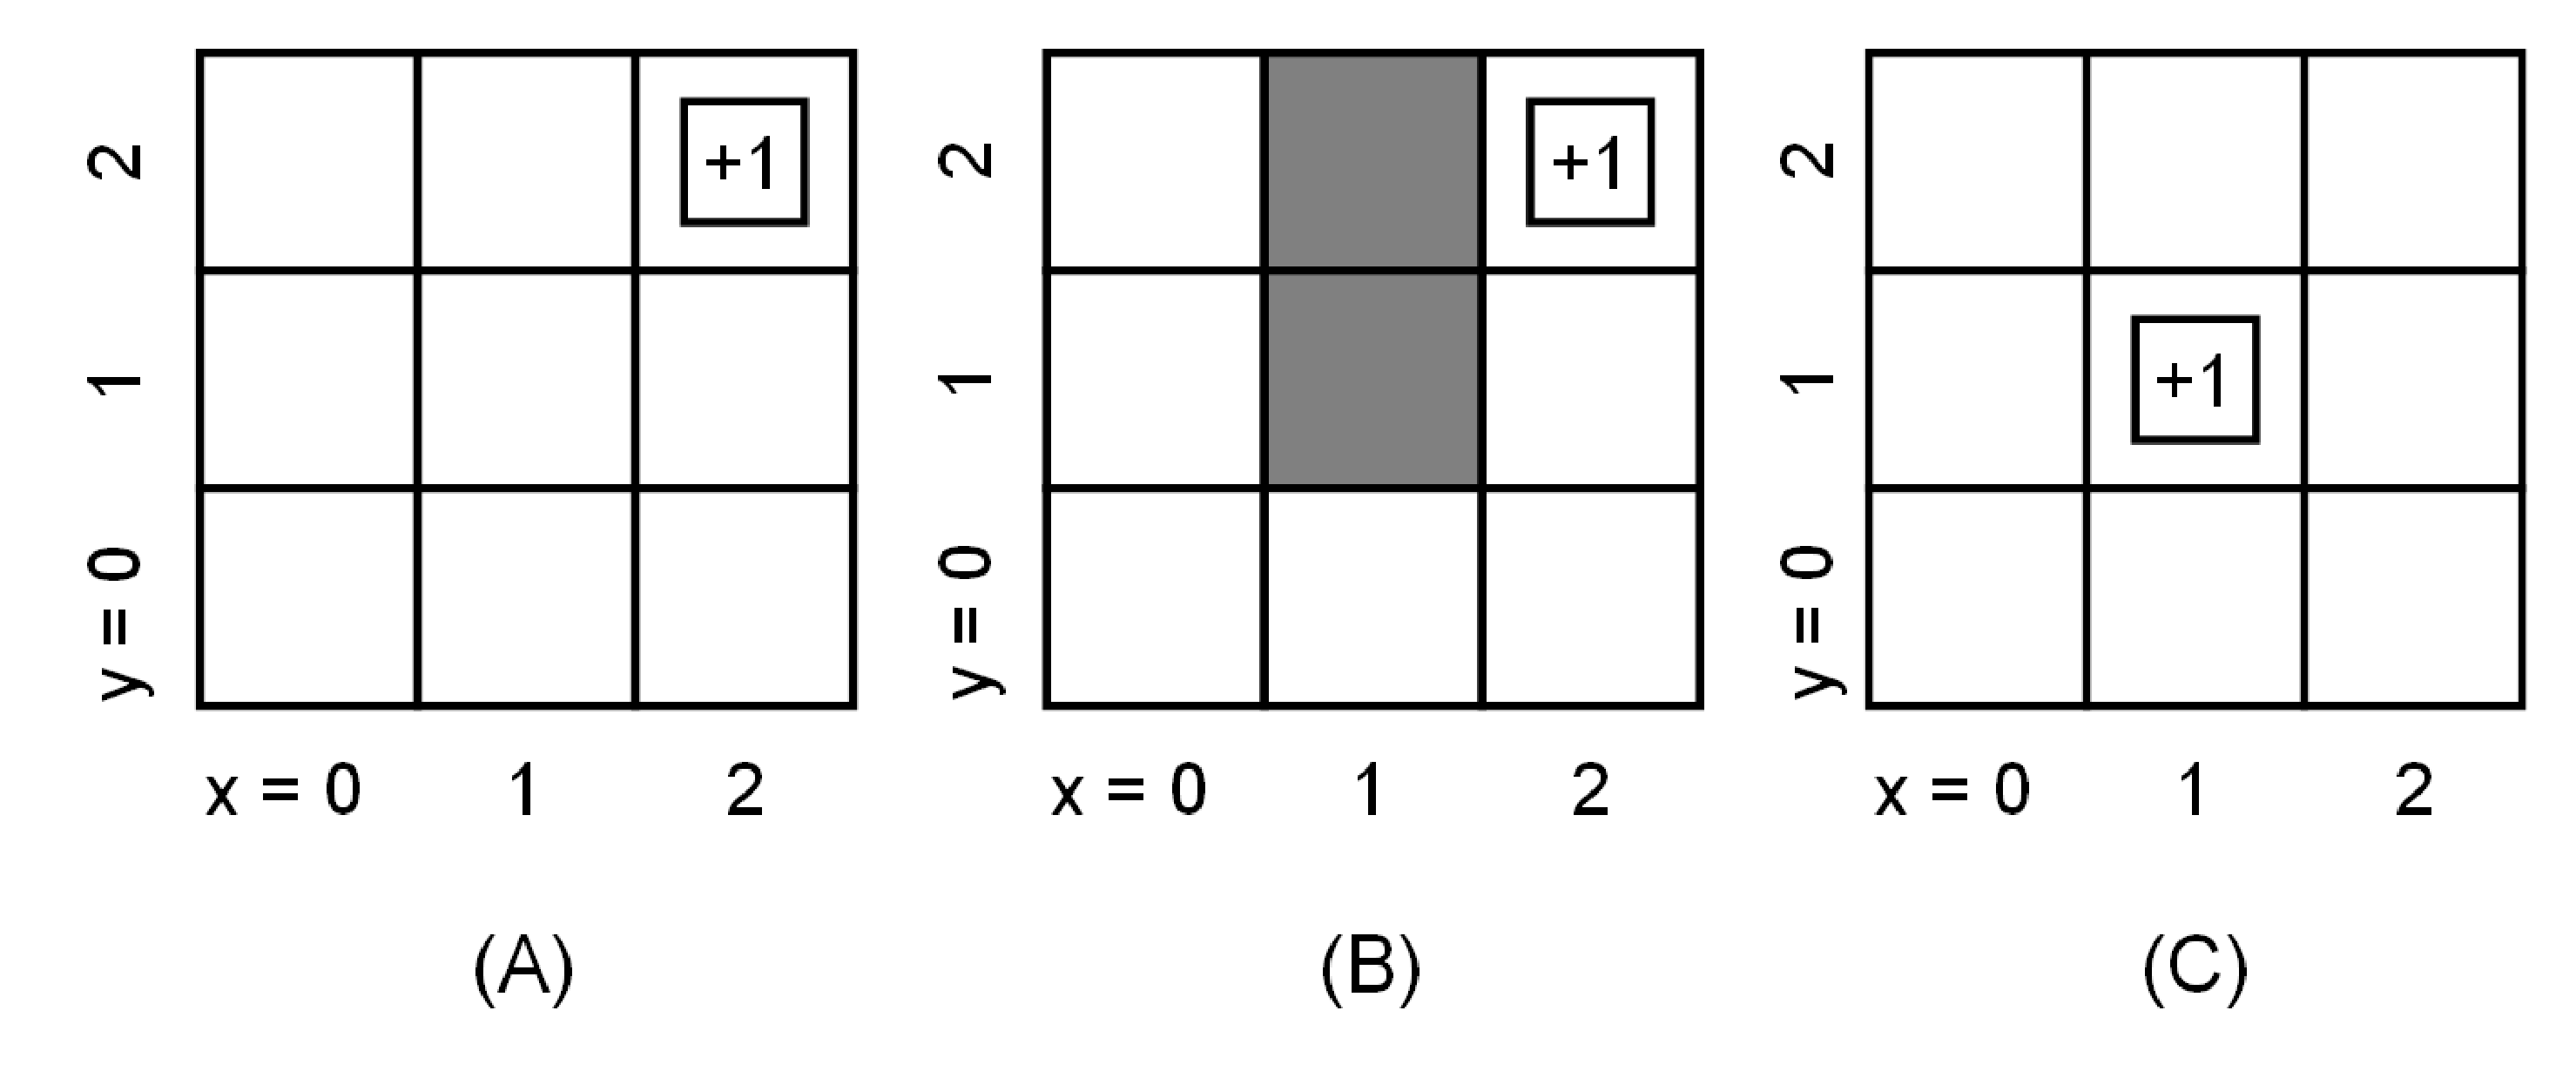
\includegraphics[width=5in]{3grid.eps}
\end{center}

\begin{enumerate}

\item Fill in the optimal values for grid (A) (hint: this should require very little calculation).

\item  Specify the optimal policy for grid (B) by placing an arrow in each empty square. \\

  Imagine we have a set of real-valued features $f_i(s)$ for each
  non-terminal state $s = (x, y)$, and we wish to approximate the
  optimal utility values $V^*(s)$ by $V(s) = \sum_i w_i \cdot f_i(s)$
  (linear feature-based approximation).

\item If our features are $f_1(x, y) = x$ and $f_2(x, y) = y$, give
  values of $w_1$ and $w_2$ for which a one-step look-ahead policy extracted
  from $V$ will be optimal in grid (A).

\item Can we represent the actual optimal values $V^*$ for grid (A)
  using these two features?  Why or why not?

\clearpage

\item For each of the feature sets listed below, state which (if any)
  of the grid MDPs above can be 'solved', in the sense that we can
  express some (possibly non-optimal) values which produce optimal
  one-step look-ahead policies.

  \begin{enumerate}

  \item $f_1(x, y) = x$ and $f_2(x, y) = y$.

  \item For each $(i, j)$, a feature $f_{i,j}(x, y) = 1$ if $(x, y) = (i, j)$, 0 otherwise.

  \item $f_1(x, y) = (x - 1)^2$, $f_2(x, y) = (y - 1)^2$, and $f_3(x, y) = 1$.

  \end{enumerate}

\end{enumerate}

\end{document}


